\documentclass[10pt,aspectratio=169,serif]{beamer}

\usepackage[fontset=none, scheme=plain]{ctex}
\IfFontExistsTF{Songti SC}{%
	\setCJKmainfont{Songti SC}[AutoFakeSlant=0.2]%
	\setCJKsansfont{Songti SC}[AutoFakeSlant=0.2]%
}{%
	\setCJKmainfont{FandolSong-Regular}[Extension=.otf,BoldFont=FandolSong-Bold,AutoFakeSlant=0.2]%
	\setCJKsansfont{FandolSong-Regular}[Extension=.otf,BoldFont=FandolSong-Bold]%
}
\usepackage{amsmath,amssymb,graphicx,tikz,booktabs,multicol,calligra}
\usepackage{pgfplots}
\pgfplotsset{compat=1.18}
\usepackage{tcolorbox}
\tcbuselibrary{skins}
\usepackage{XyygU}
\usepackage{caption}
\captionsetup[figure]{name=图,labelsep=period}

\usetikzlibrary{arrows.meta,positioning,calc}

% 公式间距
\setlength{\abovedisplayskip}{0pt plus 2pt minus 2pt}
\setlength{\belowdisplayskip}{0pt plus 2pt minus 2pt}

\title[函数的表示法练习]{函数的表示法（练习）}
\subtitle{综合运用 \& 拓广探索}
\author{}
\institute{}
\date{2026-10-15}

\begin{document}

\begin{frame}
  \titlepage
\end{frame}

% ========== 第8题 ==========
\begin{frame}[t]{第8题：矩形中的函数关系}
\textbf{8.} 如图，矩形的面积为10。如果矩形的长为 $x$，宽为 $y$，对角线为 $d$，周长为 $l$，那么你能获得关于这些量的哪些函数？

\vspace{1em}
\begin{center}
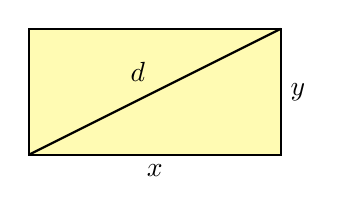
\begin{tikzpicture}[scale=0.8]
  \draw[thick,fill=yellow!30] (0,0) rectangle (4,2);
  \draw[thick] (0,0) -- (4,2);
  \node[below] at (2,0) {$x$};
  \node[right] at (4,1) {$y$};
  \node[above left] at (2,1) {$d$};
\end{tikzpicture}
\end{center}
\end{frame}

\begin{frame}[t]{第8题 解答}
\vspace{-2em}
\begin{tcolorbox}[colback=orange!10,colframe=orange,title=\textbf{解}]
由矩形面积为10，得 $xy = 10$。

\vspace{0em}
(1) 宽与长的关系：
\[
y = \frac{10}{x}, \quad x > 0.
\]
(2) 对角线与长的关系：
\[
d = \sqrt{x^2 + y^2} = \sqrt{x^2 + \frac{100}{x^2}}, \quad x > 0.
\]
(3) 周长与长的关系：
\[
l = 2(x + y) = 2\left(x + \frac{10}{x}\right), \quad x > 0.
\]
\end{tcolorbox}
\end{frame}

% ========== 第9题 ==========
\begin{frame}[t]{第9题：圆柱形容器}
\textbf{9.} 一个圆柱形容器的底部直径是 $d$ cm，高是 $h$ cm。现在向容器内每秒注入某种溶液 $v$ cm$^3$。求容器内溶液的高度 $x$（单位：cm）关于注入溶液的时间 $t$（单位：s）的函数解析式，并写出函数的定义域和值域。
\end{frame}

\begin{frame}[t]{第9题 解答}
\vspace{-2em}
\begin{tcolorbox}[colback=orange!10,colframe=orange,title=\textbf{解}]
容器底面积：
$S = \pi \left(\dfrac{d}{2}\right)^2 = \dfrac{\pi d^2}{4}.$

$t$ 秒后注入溶液体积为 $vt$，由 $vt = S \cdot x$，得：
\[
x = \frac{vt}{S} = \frac{4vt}{\pi d^2}.
\]
当溶液注满容器时，$x = h$，此时：
\[
t = \frac{h\pi d^2}{4v}.
\]
\vspace{0.5em}
\textbf{定义域：} $[0 , \dfrac{h\pi d^2}{4v}]$；
\textbf{值域：} $[0 , h]$。
\end{tcolorbox}
\end{frame}

% ========== 第10题 ==========
\begin{frame}[t]{第10题：5分制评分}
\textbf{10.} 一个老师用5分制对数学作业评分。一次作业中，第一小组同学按座位序号1，2，3，4，5，6的次序，得分依次是5，3，4，2，4，5。你会怎样表示这次作业的得分情况？用 $x$，$y$ 分别表示序号和对应的得分，$y$ 是 $x$ 的函数吗？如果是，那么它的定义域、值域和对应关系各是什么？
\end{frame}

\begin{frame}[t]{第10题 解答}
\begin{tcolorbox}[colback=orange!10,colframe=orange,title=\textbf{解}]
$y$ 是 $x$ 的函数（每个序号对应唯一得分）。

\vspace{0.5em}
\textbf{定义域：} $A = \{1, 2, 3, 4, 5, 6\}$；

\textbf{值域：} $\{2, 3, 4, 5\}$；

\textbf{对应关系：}
\[
1 \to 5,\quad 2 \to 3,\quad 3 \to 4,\quad 4 \to 2,\quad 5 \to 4,\quad 6 \to 5.
\]
\end{tcolorbox}
\end{frame}

\begin{frame}[t]{第10题 图象}
\begin{center}
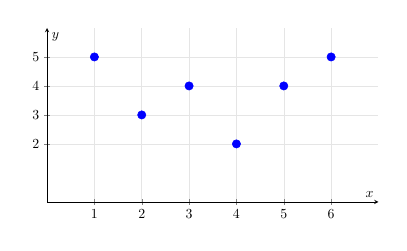
\begin{tikzpicture}[scale=0.5]
\begin{axis}[
    width=10cm, height=6cm,
    axis lines=middle,
    xlabel=$x$, ylabel=$y$,
    xmin=0, xmax=7, ymin=0, ymax=6,
    xtick={1,2,3,4,5,6},
    ytick={2,3,4,5},
    grid=major, grid style={gray!20},
]
\addplot[only marks,mark=*,mark size=3pt,blue] coordinates {(1,5)(2,3)(3,4)(4,2)(5,4)(6,5)};
\end{axis}
\end{tikzpicture}
\end{center}
\end{frame}

% ========== 第11题 ==========
\begin{frame}[t]{第11题：由图象求定义域值域}
\textbf{11.} 函数 $r = f(p)$ 的图象如图所示，
\begin{enumerate}
  \item 函数 $r = f(p)$ 的定义域、值域各是什么？
  \item $r$ 取何值时，只有唯一的 $p$ 值与之对应？
\end{enumerate}

\vspace{0.5em}
\begin{center}
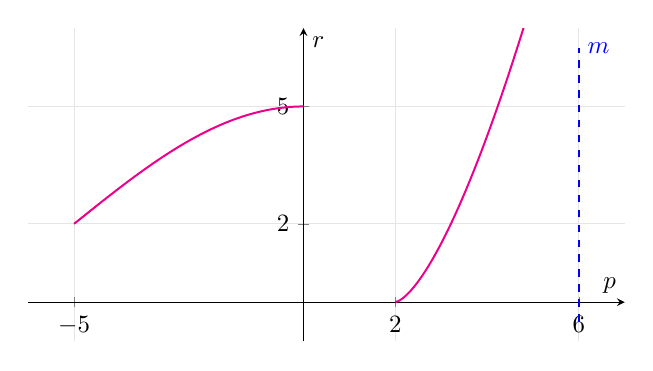
\begin{tikzpicture}[scale=0.9]
\begin{axis}[
    width=10cm, height=6cm,
    axis lines=middle,
    xlabel=$p$, ylabel=$r$,
    xmin=-6, xmax=7, ymin=-1, ymax=7,
    xtick={-5,0,2,6},
    ytick={2,5},
    grid=major, grid style={gray!20},
]
% 左边曲线：从p=-5,r=2到p=0,r=5
\addplot[thick,magenta,domain=-5:0,samples=50] {3*sin(deg((x+5)*pi/10)) + 2};
% 右边曲线：从p=2,r=0到p=6,r趋近于m=6
\addplot[thick,magenta,domain=2:6,samples=50] {1.5*(x-2)^1.5};
% 渐近线m
\draw[dashed,blue,thick] (axis cs:6,-0.5) -- (axis cs:6,6.5);
\node[right,blue] at (axis cs:6,6.5) {$m$};
\end{axis}
\end{tikzpicture}
\end{center}
\end{frame}

\begin{frame}[t]{第11题 解答}
\begin{tcolorbox}[colback=orange!10,colframe=orange,title=\textbf{解}]
(1) \textbf{定义域：} $[-5, 0] \cup [2, 6)$；

\textbf{值域：} $[0, 5] \cup [0, m)$。

(2) 当 $r \in [0, 2)$ 或 $r \in (5, m)$ 时，只有唯一的 $p$ 值与之对应。

\vspace{0.5em}
\small（因为 $r \in [2, 5]$ 时，左边曲线和右边曲线各有一个 $p$ 与之对应）
\end{tcolorbox}
\end{frame}

% ========== 第12题 ==========
\begin{frame}[t]{第12题：构造满足条件的函数}
\textbf{12.} 画出定义域为 $\{x \mid -3 \le x \le 8,\ \text{且}\ x \neq 5\}$，值域为 $\{y \mid -1 \le y \le 2,\ y \neq 0\}$ 的一个函数的图象。

\vspace{1em}
(1) 将你的图象和其他同学的相比较，有什么差别吗？

(2) 如果平面直角坐标系中点 $P(x, y)$ 的坐标满足 $-3 \le x \le 8$，$-1 \le y \le 2$，那么其中哪些点不能在图象上？
\end{frame}

\begin{frame}[t]{第12题 解答}
\begin{tcolorbox}[colback=orange!10,colframe=orange,title=\textbf{解}]
(1) 答案不唯一，只要满足：
  \begin{itemize}
    \item $x = 5$ 处没有定义（图象在 $x=5$ 处断开）；
    \item $y = 0$ 处没有函数值（图象与 $x$ 轴不相交）。
  \end{itemize}

(2) 不能在图象上的点：
  \begin{itemize}
    \item 直线 $x = 5$ 上的所有点（因为 $x \neq 5$）；
    \item 直线 $y = 0$ 上的所有点（因为 $y \neq 0$）。
  \end{itemize}
\end{tcolorbox}
\end{frame}

\begin{frame}[t]{第12题 示例图象}
\begin{center}
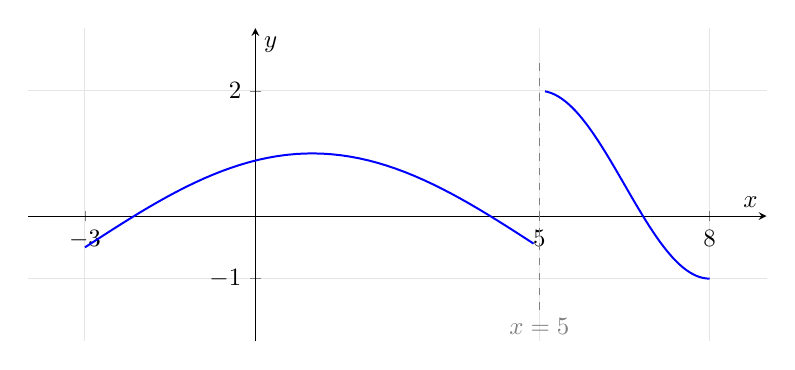
\begin{tikzpicture}[scale=0.9]
\begin{axis}[
    width=12cm, height=6cm,
    axis lines=middle,
    xlabel=$x$, ylabel=$y$,
    xmin=-4, xmax=9, ymin=-2, ymax=3,
    xtick={-3,0,5,8},
    ytick={-1,0,2},
    grid=major, grid style={gray!20},
]
% 左段：-3到5
\addplot[thick,blue,domain=-3:4.9,samples=50] {1.5*sin(deg((x+3)*pi/8)) - 0.5};
% 右段：5到8
\addplot[thick,blue,domain=5.1:8,samples=50] {1.5*cos(deg((x-5)*pi/3)) + 0.5};
% x=5处断开标记
\draw[dashed,gray] (axis cs:5,-1.5) -- (axis cs:5,2.5);
\node[below,gray] at (axis cs:5,-1.5) {$x=5$};
\end{axis}
\end{tikzpicture}
\end{center}
\end{frame}

% ========== 第13题 ==========
\begin{frame}[t]{第13题：取整函数}
\textbf{13.} 函数 $f(x) = [x]$ 的函数值表示不超过 $x$ 的最大整数，例如，$[-3.5] = -4$，$[2.1] = 2$。当 $x \in (-2.5,\ 3]$ 时，写出函数 $f(x)$ 的解析式，并画出函数的图象。
\end{frame}

\begin{frame}[t]{第13题 解答}
\begin{tcolorbox}[colback=orange!10,colframe=orange,title=\textbf{解}]
\[
f(x) =
\begin{cases}
-3, & -2.5 < x \le -2, \\
-2, & -2 < x \le -1, \\
-1, & -1 < x \le 0, \\
0, & 0 < x \le 1, \\
1, & 1 < x \le 2, \\
2, & 2 < x \le 3.
\end{cases}
\]
\end{tcolorbox}
\end{frame}

\begin{frame}[t]{第13题 图象}
\begin{center}
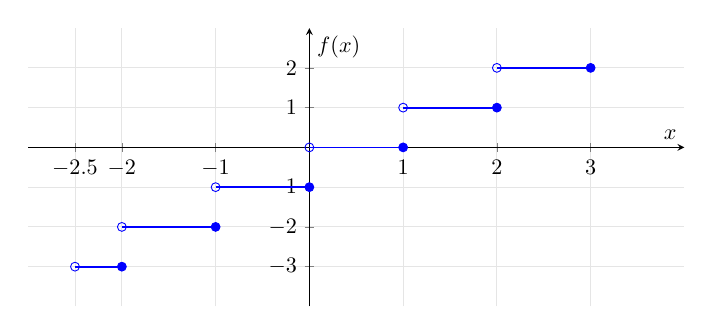
\begin{tikzpicture}[scale=0.8]
\begin{axis}[
    width=12cm, height=6cm,
    axis lines=middle,
    xlabel=$x$, ylabel=$f(x)$,
    xmin=-3, xmax=4, ymin=-4, ymax=3,
    xtick={-2.5,-2,-1,0,1,2,3},
    ytick={-3,-2,-1,0,1,2},
    grid=major, grid style={gray!20},
]
% 每个区间画水平线段
\addplot[thick,blue,domain=-2.5:-2,samples=2] {-3};
\addplot[thick,blue,domain=-2:-1,samples=2] {-2};
\addplot[thick,blue,domain=-1:0,samples=2] {-1};
\addplot[thick,blue,domain=0:1,samples=2] {0};
\addplot[thick,blue,domain=1:2,samples=2] {1};
\addplot[thick,blue,domain=2:3,samples=2] {2};
% 端点
\addplot[only marks,mark=*,mark size=2pt,blue] coordinates {(-2,-3)(-1,-2)(0,-1)(1,0)(2,1)(3,2)};
\addplot[only marks,mark=o,mark size=2pt,blue] coordinates {(-2.5,-3)(-2,-2)(-1,-1)(0,0)(1,1)(2,2)};
\end{axis}
\end{tikzpicture}
\end{center}
\end{frame}

% ========== 第14题 ==========
\begin{frame}[t]{第14题：构建问题情境}
\textbf{14.} 构建一个问题情境，使其中的变量关系能用解析式 $y = \dfrac{1}{2}ax^2\ (a > 0)$ 来描述。
\end{frame}

\begin{frame}[t]{第14题 解答}
\begin{tcolorbox}[colback=orange!10,colframe=orange,title=\textbf{参考答案}]
\textbf{情境：} 一个物体从高处自由下落，下落的距离 $y$（单位：m）与下落时间 $x$（单位：s）的关系为：
\[
y = \frac{1}{2} g x^2,
\]
其中 $g \approx 9.8\ \text{m/s}^2$ 为重力加速度。

\vspace{0.5em}
\textbf{其他情境：}
\begin{itemize}
  \item 圆的面积 $S = \pi r^2$（系数为 $\pi$）；
  \item 匀加速直线运动的位移 $s = \frac{1}{2}at^2$；
  \item 三角形面积 $S = \frac{1}{2}ah$（底一定时）。
\end{itemize}
\end{tcolorbox}
\end{frame}

% ========== 第15题 ==========
\begin{frame}[t]{第15题：小岛到城镇的时间}
\textbf{15.} 如图所示，一座小岛距离海岸线上最近的点 $P$ 的距离是 $2$ km，从点 $P$ 沿海岸正东 $12$ km 处有一个城镇。

(1) 假设一个人驾驶的小船的平均速度为 $3$ km/h，步行的速度是 $5$ km/h，$t$（单位：h）表示他从小岛到城镇的时间，$x$（单位：km）表示此人将船停在海岸处距点 $P$ 的距离。请将 $t$ 表示为 $x$ 的函数。

(2) 如果将船停在距点 $P$ $4$ km 处，那么从小岛到城镇要多长时间（精确到 $0.1$ h）？
\end{frame}

\begin{frame}[t]{第15题 配图}
\begin{center}
\begin{tikzpicture}[scale=1.2]
  % 海岸线
  \draw[thick] (-1.5,0) -- (10.5,0);

  % 小岛（蓝色圆点）
  \fill[blue!40] (0,-2) circle (0.15);
  \node[below] at (0,-2) {小岛};

  % P点
  \fill[black] (0,0) circle (2pt);
  \node[above] at (0,0) {$P$};

  % 停船点
  \fill[black] (5,0) circle (2pt);
  \node[above] at (5,0) {停船点};

  % 城镇
  \fill[black] (9,0) circle (2pt);
  \node[above] at (9,0) {城镇};

  % 垂直虚线（小岛到海岸）
  \draw[dashed] (0,0) -- (0,-2);
  \node[left] at (0,-1) {$2\,\text{km}$};

  % 直角标记
  \draw (0,-0.1) -- (0.1,-0.1) -- (0.1,0);

  % 乘船路线（虚线）
  \draw[dashed,blue,thick] (0,-2) -- (5,0);
  \node[below right,blue] at (2.5,-1) {$d_1$};

  % 距离标注：P到停船点
  \draw[<->,gray!60] (0,-0.4) -- (5,-0.4);
  \node[below,gray] at (2.5,-0.4) {$x$};

  % 距离标注：停船点到城镇
  \draw[<->,gray!60] (5,-0.4) -- (9,-0.4);
  \node[below,gray] at (7,-0.4) {$12-x$};

  % 总距离标注
  \draw[<->,gray!60] (0,-1) -- (9,-1);
  \node[below,gray] at (4.5,-1) {$12\,\text{km}$};
  \draw (5,0) -- (5,-0.5);
  \draw (9,0) -- (9,-1);
\end{tikzpicture}
\end{center}
\end{frame}

\begin{frame}[t]{第15题 解答}
\begin{tcolorbox}[colback=orange!10,colframe=orange,title=\textbf{解：(1)}]
乘船距离：$d_1 = \sqrt{x^2 + 2^2} = \sqrt{x^2 + 4}$。

乘船时间：$\dfrac{d_1}{3} = \dfrac{\sqrt{x^2 + 4}}{3}$。

步行距离：$12 - x$。

步行时间：$\dfrac{12 - x}{5}$。

\vspace{0.5em}
所以：
\[
t(x) = \frac{\sqrt{x^2 + 4}}{3} + \frac{12 - x}{5}, \quad 0 \le x \le 12.
\]
\end{tcolorbox}
\end{frame}

\begin{frame}[t]{第15题 解答：(2)}
\begin{tcolorbox}[colback=orange!10,colframe=orange,title=\textbf{解：(2)}]
当 $x = 4$ 时：
\[
t(4) = \frac{\sqrt{4^2 + 4}}{3} + \frac{12 - 4}{5} = \frac{\sqrt{20}}{3} + \frac{8}{5}.
\]

\[
\approx \frac{4.47}{3} + 1.6 \approx 1.49 + 1.6 = 3.1\ \text{h}.
\]

\vspace{0.5em}
所以从小岛到城镇约需 $\alert{3.1}$ 小时。
\end{tcolorbox}
\end{frame}

% ========== 第16题 ==========
\begin{frame}[t]{第16题：判断是否为函数}
\textbf{16.} 给定数集 $A = \mathbf{R}$，$B = (-\infty, 0]$，方程
\[
u^2 + 2v = 0. \quad \text{①}
\]

(1) 任给 $u \in A$，对应关系 $f$ 使方程①的解 $v$ 与 $u$ 对应，判断 $v = f(u)$ 是否为函数；

(2) 任给 $v \in B$，对应关系 $g$ 使方程①的解 $u$ 与 $v$ 对应，判断 $u = g(v)$ 是否为函数。
\end{frame}

\begin{frame}[t]{第16题 解答}
\begin{tcolorbox}[colback=orange!10,colframe=orange,title=\textbf{解}]
由方程 $u^2 + 2v = 0$，得 $v = -\dfrac{u^2}{2}$。

\vspace{0.5em}
(1) 对于任意 $u \in \mathbf{R}$，$v = -\dfrac{u^2}{2}$ 是唯一确定的，所以 $v = f(u)$ \alert{是}函数。

\vspace{0.5em}
(2) 由 $u^2 = -2v$，得 $u = \pm\sqrt{-2v}$。当 $v < 0$ 时，$u$ 有两个值（$\sqrt{-2v}$ 和 $-\sqrt{-2v}$）与之对应，不唯一，所以 $u = g(v)$ \alert{不是}函数。
\end{tcolorbox}
\end{frame}

% ========== 第17题 ==========
\begin{frame}[t]{第17题：探究函数}
\textbf{17.} 探究是否存在函数 $f(x)$，$g(x)$ 满足条件：

(1) 定义域相同，值域相同，但对应关系不同；

(2) 值域相同，对应关系相同，但定义域不同。
\end{frame}

\begin{frame}[t]{第17题 解答}
\begin{tcolorbox}[colback=orange!10,colframe=orange,title=\textbf{解}]
(1) \alert{存在}。例如：
\[
f(x) = x,\quad x \in [0,1],
\]
\[
g(x) = \sqrt{x},\quad x \in [0,1].
\]
定义域都是 $[0,1]$，值域都是 $[0,1]$，但对应关系不同。

\vspace{0.5em}
(2) \alert{存在}。例如：
\[
f(x) = x^2,\quad x \in \mathbf{R},
\]
\[
g(x) = x^2,\quad x \in [0, +\infty).
\]
值域都是 $[0, +\infty)$，对应关系相同（平方），但定义域不同。
\end{tcolorbox}
\end{frame}

% ========== 第18题 ==========
\begin{frame}[t]{第18题：圆周率中的数字}
\textbf{18.} 在一个展现人脑智力的综艺节目中，一位参加节目的少年能将圆周率 $\pi$ 准确地记忆到小数点后面200位，更神奇的是，当主持人说出小数点后面的位数时，这位少年都能准确地说出该数位上的数字。如果记圆周率 $\pi$ 小数点后第 $n$ 位上的数字为 $y$，那么你认为 $y$ 是 $n$ 的函数吗？如果是，请写出函数的定义域、值域与对应关系；如果不是，请说明理由。
\end{frame}

\begin{frame}[t]{第18题 解答}
\begin{tcolorbox}[colback=orange!10,colframe=orange,title=\textbf{解}]
$y$ 是 $n$ 的函数。

\vspace{0.5em}
\textbf{定义域：} $\{n \mid 1 \le n \le 200,\ n \in \mathbf{N}^*\}$；

\textbf{值域：} $\{0, 1, 2, 3, 4, 5, 6, 7, 8, 9\}$；

\textbf{对应关系：} $y$ 等于圆周率 $\pi$ 小数点后第 $n$ 位上的数字。

\vspace{0.5em}
（每个 $n$ 对应唯一的数字，满足函数定义）
\end{tcolorbox}
\end{frame}

\begin{frame}[c]
  \begin{center}
    {\Huge\calligra Thanks!}
  \end{center}
\end{frame}

\end{document}
